%!TEX root = ./ERL Industrial Robots.tex

%--------------------------------------------------------------------
%--------------------------------------------------------------------
\subsection{Task \emph{Prepare Assembly Aid Tray for Force Fitting}}
\label{ssec:TaskAssemblyAidTray}

This task serves as an example for collecting and assembling parts from different locations. 
Additionally, the teams can show their robots capability in loading and unloading machines (a well known industrial task).
Figure \ref{fig:AidTrayRack} shows the aid tray rack used in the benchmark. On the side of the aid tray unique identifiers are visible to identify the object.
The aid tray is a container that can store up to two bearing boxes.

\begin{figure}[!htbp]
	\begin{center}
		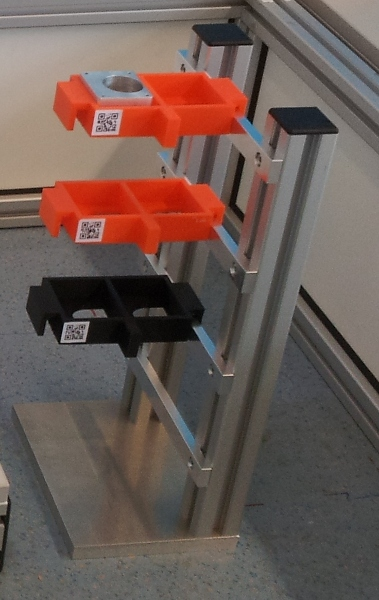
\includegraphics[scale=0.5,angle=0]{pics/atwork/arena_elements/Aid_tray_rack}
		\caption{\roaw Aid tray rack.}
		\label{fig:AidTrayRack}
	\end{center}
\end{figure}

%--------------------------------------------------------------------
\subsubsection{Task Description}
\label{sssec:TaskAssemblyAidTrayDescription}

The robots task is to assist the force fitting process of bearings into bearing boxes with the help of assembly aid tray and force fitting machine. 

%--------------------------------------------------------------------
\subsubsection{Feature Variation}
\label{sssec:TaskAssemblyAidTrayVariation}

The bearing boxes can occur in different shapes (see list of parts in Table \ref{tab:DriveAxlePartsRulebook}). This is caused by a modular concept of the final product where the bearing box has to be inserted in different chassis.
The robots are allowed to collect and insert the bearing boxes in the assembly aid tray individually or collectively.

%--------------------------------------------------------------------
\subsubsection{Input Provided}
\label{sssec:TaskAssemblyAidTrayInput}

The team will be provided with the following information:

\begin{itemize}
\item description of the set of possible assembly aid tray and bearing boxes.
\item description and location(s) of the container(s) used for the bearing boxes.
\end{itemize}

During the execution of the task, the robot should perform the task autonomously and without any additional input.

%--------------------------------------------------------------------
\subsubsection{Expected Robot Behavior or Output}
\label{sssec:TaskAssemblyAidTrayOutput}

The robot navigates to the storage area and collects bearing boxes to be placed into the assembly aid tray.
The robot has the option to deliver the bearing boxes collectively or individually.
After placing the bearing boxes in the assembly aid tray, the robot delivers the assembly aid tray to the force fitting workstation. 
In the force fitting workstation, the assembly aid tray will be processed and the robot will be informed when the process is completed.
The robot will check the final product and can request for another force fitting process when the result is unsatisfactory.

%--------------------------------------------------------------------
\subsubsection{Procedures and Rules}
\label{sssec:TaskAssemblyAidTrayProcedures}

During the execution of this task, which needs to be carried out as per the next steps, an additional robot might be randomly moving in the arena which has to be avoided by the participating robot. 

\begin{description}
     \item [Step 1] The robot, through communicating with the CFH, is provided with multiple assembly aid trays and the information regarding the storage area of the bearing boxes.
     \item [Step 2] Based on the identifier provided beforehand to the teams, the robot must identify the appropriate bearing boxes needed to be put on a tray.
     \item [Step 3] The robot must pick and insert the bearing boxes, identified in Step 2 above, in the provided assembly aid tray.
     \item [Step 4] The robot must deliver the assembly aid tray (with the bearing boxes) to the force fitting workstation to be processed.
\end{description}

%--------------------------------------------------------------------
\subsubsection{Communication to CFH}
\label{sssec:CommCFH}

For this task benchmark the robot does not have to control any networked device in the environment. The force fitting machine will be operated by a human worker. All necessary CFH communication is described in Section \ref{sec:CommCFH}.

%--------------------------------------------------------------------
\subsubsection{Acquisition of Benchmarking Data}
\label{sssec:TaskAssemblyAidTrayData}

General information on the acquisition of benchmarking data is described in Section \ref{sec:TbmAcquisitionOfData}. There, the \textbf{offline} part of the benchmarking data can be found.

\paragraph{Online data}
In order to send online benchmarking data to the CFH, the robot has to use the \textbf{BenchmarkFeedback} message. The message contains:
\begin{itemize}
\item assembly\_aid\_tray\_id (type: string)
\item container\_id (type: string)
\end{itemize}

\paragraph{Offline data} 
The additional information described in the following table has to be logged:

\begin{table}[h]
	\centering
	\begin{footnotesize}
		\begin{tabular}{|l|l|l|l|}
			\hline
			Topic	&	Type		&	Frame Id		&	Notes \\ \hline\hline
			/rockin/qrcode\tablefootnote{ID of the assembly aid tray or container, detected by the robot by analyzing the QR code.} & std\_msgs/Int32 & -- & when recognized \\ \hline
		\end{tabular}
	\end{footnotesize}
\end{table}


%--------------------------------------------------------------------
\subsubsection{Scoring and Ranking}
\label{sssec:TaskAssemblyAidTrayScoring}

Evaluation of the performance of a robot according to this task benchmark is based on performance equivalence classes. Classes are defined in dependence to:

\begin{enumerate}
\item The fact that the robot correctly identifies the assembly aid tray or not;
\item The number of bearing boxes successfully inserted by the robot into the aid tray;
\item The successful execution of the force fitting procedure.
\end{enumerate}

\noindent 
\paragraph{Achievements} The set $A$ of achievements for this task includes:
\begin{itemize}
\item The robot correctly identifies the assembly aid trays identifier.
\item The robot correctly grasps the assembly aid tray.
\item The robot correctly grasps the first bearing box.
\item The robot correctly grasps the second bearing box.
\item The robot inserts the first bearing box into the aid tray.
\item The robot inserts the second bearing box into the aid tray.
\item The robot correctly delivers the tray to the force fitting station.
\item The robot completely processes the first bearing (from identifying to delivering).
\item The robot completely processes the second bearing (from identifying to delivering).
\item The robot cooperates with CFH and Networked Devices throughout the task.
\item The team delivers the benchmarking data appropriately.
\end{itemize}
%--------------------------------------------------------------------
% EOF
%--------------------------------------------------------------------
